\section{Thermal Expansion} \index{Thermal expansion}

\begin{multicols}{2}


\subsection{Explaining Expansion}

\begin{center}
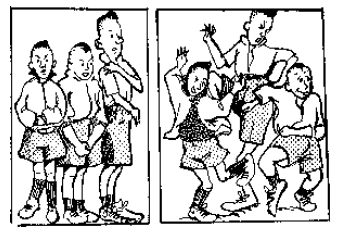
\includegraphics[width=0.4\textwidth]{./img/source/explaining-expansion-2.png}
\end{center}

\begin{description*}
%\item[Subtopic:]{}
%\item[Materials:]{}
%\item[Setup:]{}
%\item[Procedure:]{}
%\item[Hazards:]{}
%\item[Questions:]{}
%\item[Observations:]{}
\item[Theory:]{Expansion can be explained by a simple human model: When a group of students stands still, they are close together and they do not need much space. But if they start to dance or run about, each of them needs more space and the group as a whole takes more space. The particles in a body are like the students, they only move far apart when they are heated and hence need more space.}
%\item[Applications:]{}
%\item[Notes:]{}
\end{description*}


\section*{Thermal Expansion of Solids} \index{Thermal expansion! of solids}


\subsection{Ring and Nail}

\begin{center}
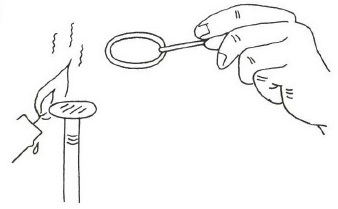
\includegraphics[width=0.4\textwidth]{./img/vso/ring-nail.jpg}
\end{center}

\begin{description*}
%\item[Subtopic:]{}
\item[Materials:]{Nail, wire (10 cm), candle}
%\item[Setup:]{}
\item[Procedure:]{Make a wire loop which is just big enough to pass over the head of the nail. Heat the nail.}
%\item[Hazards:]{}
%\item[Questions:]{}
\item[Observations:]{After heating, the loop no longer fits over the head of the nail.}
\item[Theory:]{Heating the nail causes it to expand, and thus the loop can no longer fit over the hot nail head.}
%\item[Applications:]{}
%\item[Notes:]{}
\end{description*}

\subsection{Expansion of a Coin}

\begin{center}
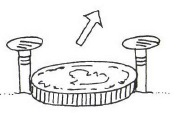
\includegraphics[width=0.3\textwidth]{./img/vso/expansion-coin.jpg}
\end{center}

\begin{description*}
%\item[Subtopic:]{}
\item[Materials:]{Coin, 2 nails, mounting board/cardboard, candle}
%\item[Setup:]{}
\item[Procedure:]{Place the coin between the nails, then heat the nails.}
%\item[Hazards:]{}
%\item[Questions:]{}
\item[Observations:]{The coin cannot be removed after heating the nails.}
\item[Theory:]{Metals expand when heated, thus the nails expand and fit tightly around the coin.}
%\item[Applications:]{}
%\item[Notes:]{}
\end{description*}

\subsection{Expansion of a Wire}

\begin{center}
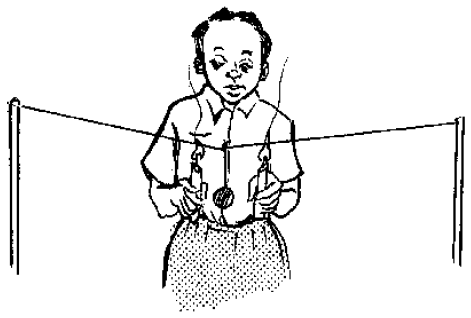
\includegraphics[width=0.4\textwidth]{./img/source/expansion-wire.png}
\end{center}

\begin{description*}
%\item[Subtopic:]{}
\item[Materials:]{Copper wire, chairs, small weight, candle}
%\item[Setup:]{}
\item[Procedure:]{Fix a thin copper wire between two chairs and hang a weight in the middle to stretch the wire. Then heat the wire along its length.}
%\item[Hazards:]{}
%\item[Questions:]{}
\item[Observations:]{The weight sags further down upon heating the wire.}
\item[Theory:]{The heated wire expands and hence increases its length.}
%\item[Applications:]{}
%\item[Notes:]{}
\end{description*}

\columnbreak

\subsection{Breaking Glass}

%\begin{center}
%\includegraphics[width=0.4\textwidth]{./img/source/.png}
%\end{center}

\begin{description*}
%\item[Subtopic:]{}
\item[Materials:]{Soda bottle, water, \nameref{sec:heatsources}}
%\item[Setup:]{}
\item[Procedure:]{Fill an open glass container about half way with water. Place the bottle over a heat source and wait. If the bottle does not break before the water boils, remove it and place it in a bath of cold water.}
\item[Hazards:]{Be sure the bottle is not covered when heating. If covered, the bottle can explode rather than break evenly.}
%\item[Questions:]{}
\item[Observations:]{The bottle breaks evenly at the level of the water inside.}
\item[Theory:]{The water in the bottle gains more heat than the air above it, so the glass touching the water also gains more heat and thus expands more than the glass above the water. As a result, the glass breaks evenly.}
%\item[Applications:]{}
%\item[Notes:]{}
\end{description*}

\subsection{Thermal Switch}

\begin{center}
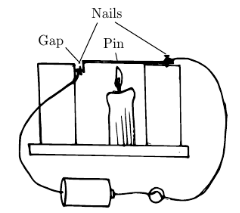
\includegraphics[width=0.4\textwidth]{./img/thermal-switch.png}
\end{center}

\begin{description*}
%\item[Subtopic:]{}
\item[Materials:]{Piece of wood, 2 thick sticks (5 cm tall), several small nails, pin, connecting wires, 2 dry cells, bulb or galvanometer, candle}
\item[Setup:]{Nail the sticks upright on the wood, a few cm apart. Fix one nail horizontally near the top of one stick. Bend the end of the pin (half cm) at a right angle and place on top of the other stick so that the bent end just touches the horizontal nail. Move the pin back slightly to leave a small gap and fix it in place with another nail. Attach connecting wires to the back end of the pin and the opposite nail, and connect in series with to a bulb/galvanometer and dry cells.}
\item[Procedure:]{Heat the pin until it touches the horizontal nail.}
%\item[Hazards:]{}
%\item[Questions:]{}
\item[Observations:]{The bulb lights or the galvanometer shows a deflection.}
\item[Theory:]{Heating the pin causes it to expand and thus close the circuit, allowing current to flow.}
%\item[Applications:]{}
%\item[Notes:]{}
\end{description*}

\subsection{Bimetallic Strip}

\begin{center}
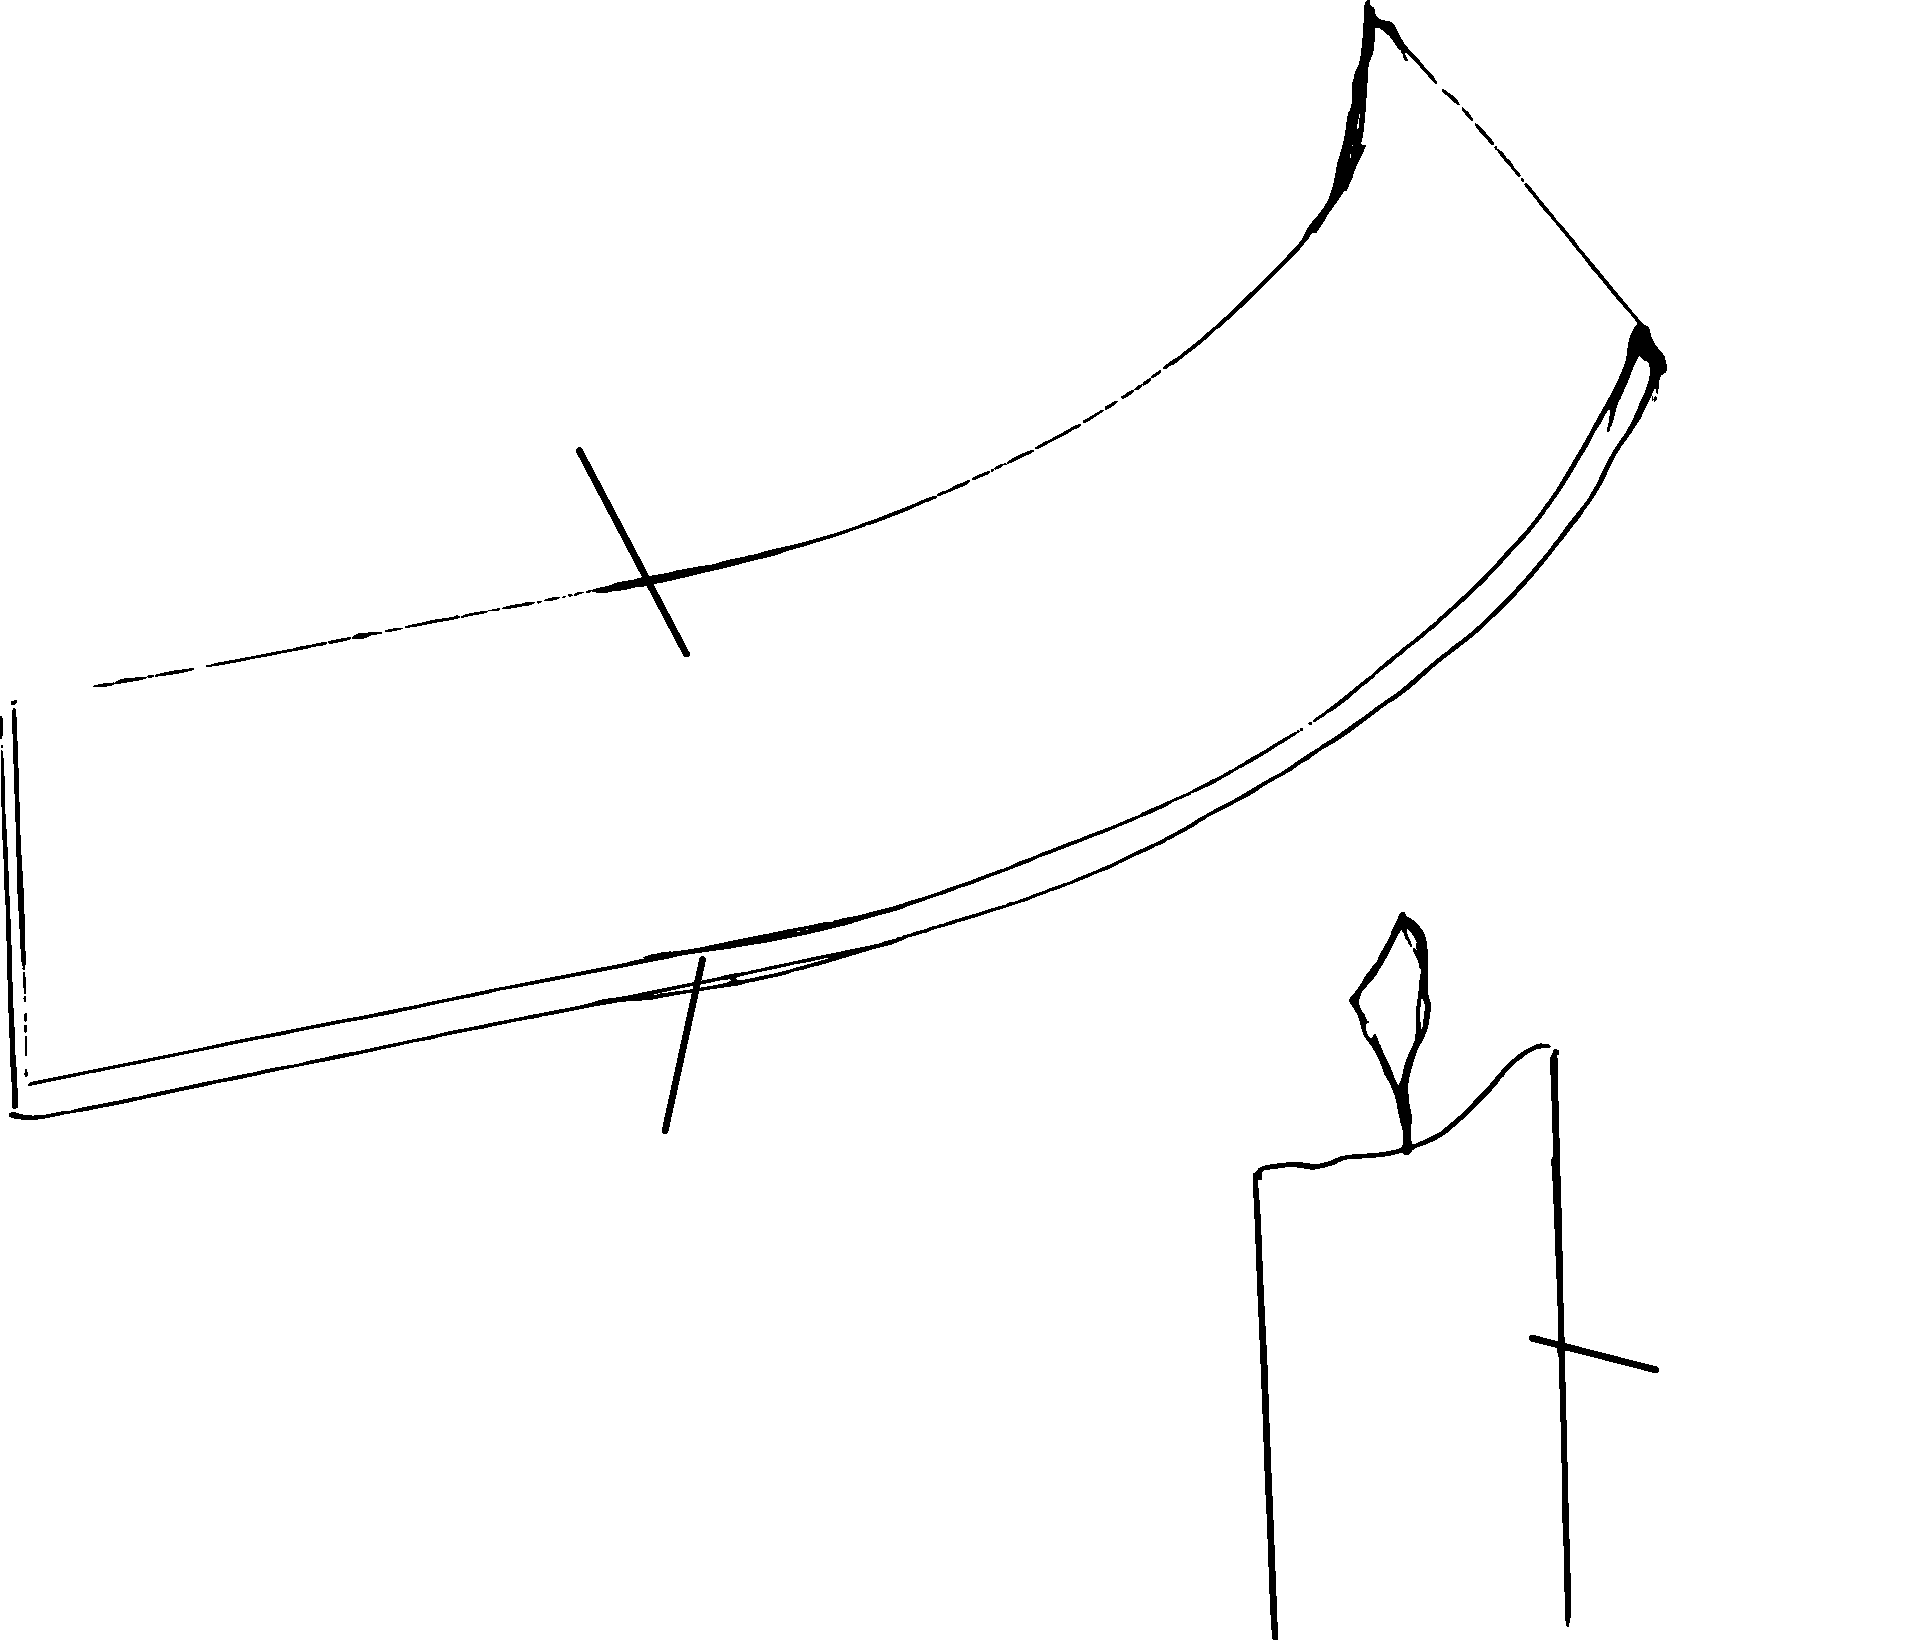
\includegraphics[width=0.4\textwidth]{./img/bimetallic-strip.png}
\end{center}

\begin{description*}
%\item[Subtopic:]{}
\item[Materials:]{Strip of paper, aluminum foil, glue, candle}
\item[Setup:]{Cut equal size pieces of aluminum foil and paper (about 3 cm $\times$ 10 cm). Glue the two pieces together.}
\item[Procedure:]{Place the bimetallic strip over a flame. Try heating either side.}
%\item[Hazards:]{}
%\item[Questions:]{}
\item[Observations:]{The strip bends towards the paper side.}
\item[Theory:]{Aluminum expands more than paper, so the aluminum side becomes longer than the paper side.}
%\item[Applications:]{}
%\item[Notes:]{}
\end{description*}

\subsection{Measuring Expansion}

\begin{center}
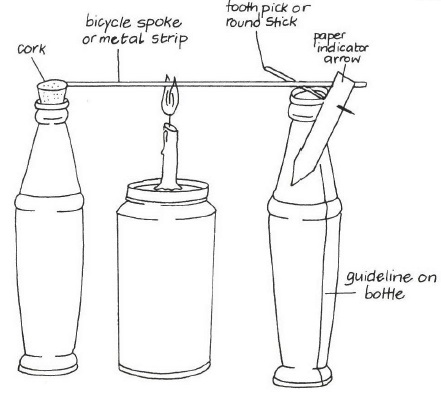
\includegraphics[width=0.49\textwidth]{./img/vso/measuring-expansion.jpg}
\end{center}

\begin{description*}
%\item[Subtopic:]{}
\item[Materials:]{2 bottles, cork/rubber stopper, bicycle spoke/thick wire, candle, toothpick, paper}
\item[Setup:]{Push the spoke into the cork so that it is held firmly. Arrange the rest of the equipment as shown.}
\item[Procedure:]{Heat the spoke and observe the paper indicator arrow.}
%\item[Hazards:]{}
%\item[Questions:]{}
\item[Observations:]{As the metal is heated it expands and the indicator moves.}
%\item[Theory:]{}
%\item[Applications:]{}
%\item[Notes:]{}
\end{description*}

\subsection{Allowing for Expansion}

\begin{center}
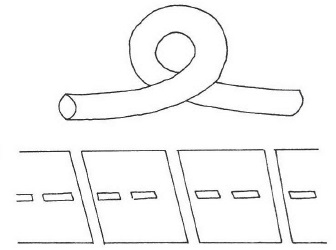
\includegraphics[width=0.4\textwidth]{./img/vso/allowing-expansion.jpg}
\end{center}

\begin{description*}
%\item[Subtopic:]{}
%\item[Materials:]{}
%\item[Setup:]{}
%\item[Procedure:]{}
%\item[Hazards:]{}
%\item[Questions:]{}
%\item[Observations:]{}
%\item[Theory:]{}
\item[Applications:]{Steam and oil pipelines in hot areas often have loops to allow for expansion and contraction. Slabs on a concrete road have gaps between them to allow them to expand in the heat. Tar is put into the gaps because it is flexible.}
%\item[Notes:]{}
\end{description*}

%==================================================================================================%

\section*{Thermal Expansion of Liquids} \index{Thermal expansion! of liquids}


\subsection{Rising Colours}

\begin{center}
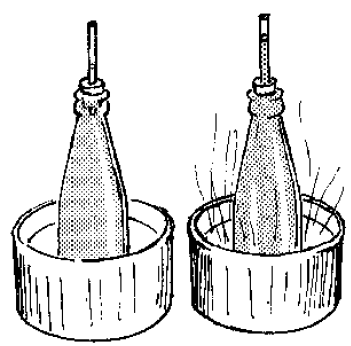
\includegraphics[width=0.4\textwidth]{./img/source/rising-colours.png}
\end{center}

\begin{description*}
%\item[Subtopic:]{}
\item[Materials:]{Bottle, cork/stopper, pen tube, water, food colour, container, \nameref{sec:heatsources}}
%\item[Setup:]{}
\item[Procedure:]{Fill a bottle to the rim with coloured water. Tightly fix a cork bearing a transparent hollow pen tube. Place the bottle in hot water.}
%\item[Hazards:]{}
%\item[Questions:]{}
%\item[Observations:]{}
\item[Theory:]{The liquid rises in the tube because it is heated by the hot water and expands.}
\item[Applications:]{Mark even intervals on the pen tube to make a simple thermometer.}
%\item[Notes:]{}
\end{description*}

\subsection{Jumping Coin}

\begin{center}
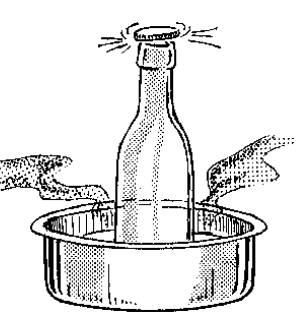
\includegraphics[width=0.35\textwidth]{./img/source/jumping-coin.png}
\end{center}

\begin{description*}
%\item[Subtopic:]{}
\item[Materials:]{Bottle, coin, container, \nameref{sec:heatsources}}
%\item[Setup:]{}
\item[Procedure:]{Wet the rim of a bottle with water and cover it with a coin. Place the bottle into a hot water bath.}
%\item[Hazards:]{}
%\item[Questions:]{}
\item[Observations:]{The coin vibrates, opening and closing the bottle.}
\item[Theory:]{When the air in the bottle expands, it pushes up on the coin, and when the air escapes, the pressure inside drops and the atmospheric pressure pushes down on the coin.}
%\item[Applications:]{}
%\item[Notes:]{}
\end{description*}

\subsection{Liquid Thermometers} \index{Thermometer}

\begin{center}
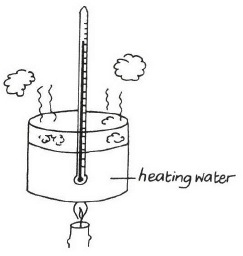
\includegraphics[width=0.4\textwidth]{./img/vso/liquid-thermometers.jpg}
\end{center}

\begin{description*}
%\item[Subtopic:]{}
%\item[Materials:]{}
%\item[Setup:]{}
%\item[Procedure:]{}
%\item[Hazards:]{}
%\item[Questions:]{}
%\item[Observations:]{}
%\item[Theory:]{}
\item[Applications:]{The mercury or alcohol expands and contracts according to its temperature.}
%\item[Notes:]{}
\end{description*}

\subsection[Allowing for Liquid Expansion]{Allowing for Liquid \hfill \\ Expansion}

\begin{center}
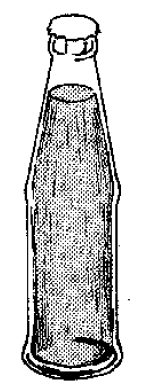
\includegraphics[width=0.1\textwidth]{./img/source/allowing-expansion-liquid.png}
\end{center}

\begin{description*}
%\item[Subtopic:]{}
%\item[Materials:]{}
%\item[Setup:]{}
%\item[Procedure:]{}
%\item[Hazards:]{}
\item[Observations:]{Observe the liquid level at the top of an unopened soda or beer bottle.}
\item[Questions:]{Why does the bottle contain a small amount of gas trapped above the soda or beer?}
\item[Theory:]{The space is to allow the expansion of soda or beer when the bottle is stored in a warm place.}
%\item[Applications:]{}
%\item[Notes:]{}
\end{description*}

%==================================================================================================%

\section*{Thermal Expansion of Gases} \index{Thermal expansion! of gases}
%\textbf{Charles' Law} states that the volume of a fixed mass of a gas is directly proportional to the temperature provided the pressure remains constant. ($V \propto T$ at constant $P$)\\
%\textbf{Boyle's Law} state that the volume of a fixed mass of gas is inversely proportional to its pressure if the temperature remains constant. ($V \propto \frac{1}{P}$ at constant $T$)

% Charles' Law
\subsection*{Charles' Law} \index{Charles' Law}

\subsection{Bottle Crush}

\begin{center}
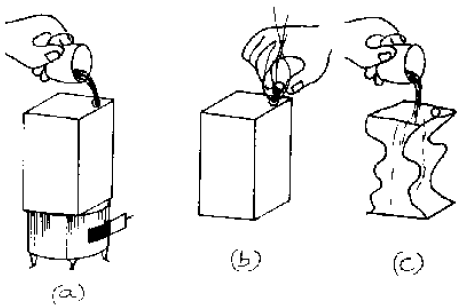
\includegraphics[width=0.45\textwidth]{./img/source/bottle-crush.png}
\end{center}

\begin{description*}
%\item[Subtopic:]{}
\item[Materials:]{Plastic water bottle, boiling water, cold water}
%\item[Setup:]{}
\item[Procedure:]{Pour some boiling water into the bottle and cap it immediately. Shake it to make sure all the air inside is heated. Pour out the hot water and cap the bottle. Then pour cold water on the outside of the bottle.}
%\item[Hazards:]{}
%\item[Questions:]{}
\item[Observations:]{Upon pouring the cold water, the bottle crushes.}
\item[Theory:]{Boiling water is used initially to increase the temperature of the air in the bottle. It is removed and the bottle is sealed, forcing the pressure to remain constant. As the air inside the bottle cools, it decreases the volume, causing the bottle to be crushed from the inside. $T \propto V$ when $P$ is constant.}
\item[Applications:]{See also \nameref{sec:atm-pressure}.}
%\item[Notes:]{This is an application of Charles' Law. For more, see \nameref{}.}
\end{description*}

\subsection{Egg Suck}

\begin{center}
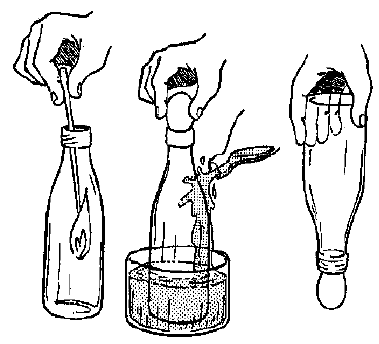
\includegraphics[width=0.4\textwidth]{./img/source/egg-suck.png}
\end{center}

\begin{description*}
%\item[Subtopic:]{}
\item[Materials:]{Bottle, wooden stick, matches, boiled egg, cold water}
\item[Setup:]{Boil and peel an egg.}
\item[Procedure:]{Place an empty bottle into a hot water bath or burn a wooden stick inside of it. After it has warmed up, close the bottle with the egg. Now immerse the bottle in cold water.}
%\item[Hazards:]{}
%\item[Questions:]{}
\item[Observations:]{The egg is held by the bottle and may even be sucked into the bottle.}
\item[Theory:]{Cooling the air in the bottle (decrease in temperature) causes it to contract (decrease in volume) and hence lowers the air pressure inside. If the pressure difference with the outside atmospheric pressure is great enough, the egg will be slowly sucked into the bottle.}
%\item[Applications:]{}
\item[Notes:]{Try to use an egg of comparable size to the opening of the bottle.}
\end{description*}

\subsection{Spray Balloon}

%\begin{center}
%\includegraphics[width=0.4\textwidth]{./img/source/.png}
%\end{center}

\begin{description*}
%\item[Subtopic:]{}
\item[Materials:]{Can of aerosol spray (e.g. Rungu insect repellent), balloon/plastic bag}
%\item[Setup:]{}
\item[Procedure:]{Place a balloon or plastic bag over the mouth of the spray can and spray into the balloon. Use a funnel if necessary to fill the balloon. Tie the balloon.}
%\item[Hazards:]{}
%\item[Questions:]{}
\item[Observations:]{The spray liquefies and is cold inside the balloon. As the liquid warms to room temperature, it changes from a liquid to a gas. Students can hear and feel it boiling. As the gas heats up, the balloon expands.}
\item[Theory:]{The spray begins as a cool liquid when released from the can. As the temperature increases to that of the room, the volume of the trapped gas also increases.}
%\item[Applications:]{}
%\item[Notes:]{}
\end{description*}

% Boyle's Law
\subsection*{Boyle's Law} \index{Boyle's Law}

\subsection{Syringe Suck}

\begin{center}
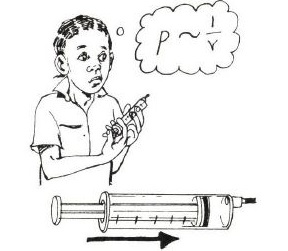
\includegraphics[width=0.45\textwidth]{./img/source/boyle-syringe.jpg}
\end{center}

\begin{description*}
%\item[Subtopic:]{}
\item[Materials:]{Syringe}
%\item[Setup:]{}
\item[Procedure:]{Fill the syringe with air and place a finger at the tip to create a seal. Press the plunger as far as possible.}
%\item[Hazards:]{}
%\item[Questions:]{}
\item[Observations:]{It is easy to decrease the volume most of the way but impossible by human means to completely remove all the air inside.}
\item[Theory:]{As you increase the pressure by pressing the plunger, the volume inside the syringe decreases. As the volume decreases, the pressure inside the syringe increases, making it increasingly difficult to continue pressing the plunger.}
%\item[Applications:]{}
%\item[Notes:]{}
\end{description*}

\vfill
\columnbreak

\subsection{Balloon Blow}

%\begin{center}
%\includegraphics[width=0.4\textwidth]{./img/source/.png}
%\end{center}

\begin{description*}
%\item[Subtopic:]{}
\item[Materials:]{Bottle, balloon}
%\item[Setup:]{}
\item[Procedure:]{Place a balloon over the mouth of a bottle so that it hangs inside the bottle. Try to blow up the balloon inside the bottle.}
%\item[Hazards:]{}
%\item[Questions:]{}
\item[Observations:]{It is impossible for a normal person to fill the balloon.}
\item[Theory:]{In order to fill the balloon, the volume of air inside the bottle must decrease. For this to happen, Boyle's Law states that the pressure must increase. A normal human's lungs cannot blow at a high enough pressure to fill the balloon inside the bottle.}
%\item[Applications:]{}
%\item[Notes:]{}
\end{description*}

\subsection{Balloon Suck}

%\begin{center}
%\includegraphics[width=0.4\textwidth]{./img/source/.png}
%\end{center}

\begin{description*}
%\item[Subtopic:]{}
\item[Materials:]{Balloon, plastic bottle, straw, super glue}
\item[Setup:]{Put a straw through the wall of a plastic bottle and seal with super glue.}
\item[Procedure:]{Place a balloon over the mouth of the bottle so that it hangs inside the bottle. Use the straw to suck air out of the bottle.}
%\item[Hazards:]{}
%\item[Questions:]{}
\item[Observations:]{As the air is sucked through the straw, the balloon fills with air.}
\item[Theory:]{Sucking air out of the bottle decreases its volume. Atmospheric pressure compensates by pushing the balloon into the bottle, which fills up with air.}
%\item[Applications:]{}
%\item[Notes:]{}
\end{description*}

%==================================================================================================%


\end{multicols}

\pagebreak